\begin{figure}
\centering
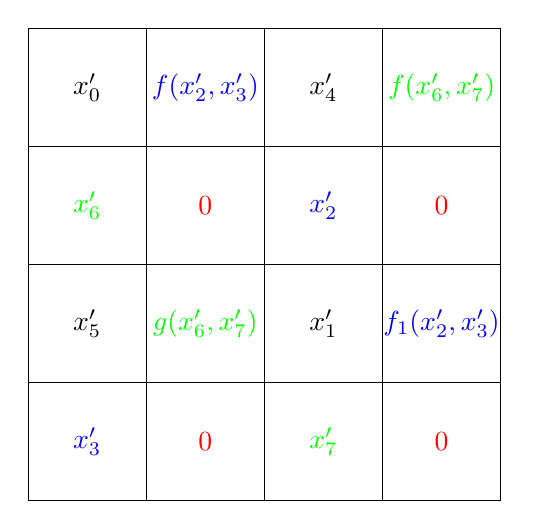
\begin{tikzpicture}[scale=1.5]
\foreach \i in {0,1,2,3}{
	\foreach \j in {0,1,2,3}{
		\draw (\i,\j) rectangle (\i + 1, \j + 1);
	}
}
\draw (.5,3.5) node {$x_0'$};
\draw (1.5,3.5) node {$\color{blue}{f(x_2',x_3')}$};
\draw (2.5,3.5) node {$x_4'$};
\draw (3.5,3.5) node {$\color{green}{f(x_6',x_7')}$};

\draw (.5,2.5) node {$\color{green}{x_6'}$};
\draw (1.5,2.5) node {$\color{red}{0}$};
\draw (2.5,2.5) node {$\color{blue}{x_2'}$};
\draw (3.5,2.5) node {$\color{red}{0}$};

\draw (.5,1.5) node {$x_5'$};
\draw (1.5,1.5) node {$\color{green}{g(x_6',x_7')}$};
\draw (2.5,1.5) node {$x_1'$};
\draw (3.5,1.5) node {$\color{blue}{f_1(x_2',x_3')}$};

\draw (.5,.5) node {$\color{blue}{x_3'}$};
\draw (1.5,.5) node {$\color{red}{0}$};
\draw (2.5,.5) node {$\color{green}{x_7'}$};
\draw (3.5,.5) node {$\color{red}{0}$};
\end{tikzpicture}
\caption{Possible states for $\delta^4$}
\label{fig:solutiondelta4}
\end{figure}